% --------------------------------------------------------------------------
%\documentclass[onecolumn,11pt]{ieeetran}
%\documentclass[draft]{siamltex}
\documentclass[11pt]{article}
\usepackage{graphics,stfloats,amssymb,amsmath,amsfonts,epsfig}
\usepackage{algorithm}
\usepackage{algorithmic}
\usepackage{hyperref}
\usepackage{verbatim}
%\usepackage[named]{algo}

% Example definitions
% -------------------
\def\x{{\mathbf x}}
\def\L{{\cal L}}
\def\half{\frac{1}{2}}
\def\alphamax{\alpha_{\mbox{\tiny max}}}
\def\alphamin{\alpha_{\mbox{\tiny min}}}


% more useful abbreviations
% -------------------------
\newcommand{\R}{\mathbb{R}}
\newcommand{\C}{\mathbb{C}}
\newcommand{\btheta}{\mbox{\boldmath $\theta$}}
\newcommand{\bgamma}{\mbox{\boldmath $\gamma$}}
\newcommand{\bbeta}{\mbox{\boldmath  $\beta$}}
\newcommand{\balpha}{\mbox{\boldmath $\alpha$}}
\newcommand{\bDelta}{\mbox{\boldmath $\Delta$}}
\newcommand{\bdelta}{\mbox{\boldmath $\delta$}}
\newcommand{\bPsi}{\mbox{\boldmath   $\Psi$}}
\newcommand{\bphi}{\mbox{\boldmath   $\phi$}}
\newcommand{\bpi}{\mbox{\boldmath    $\pi$}}
\newcommand{\btau}{\mbox{\boldmath   $\tau$}}
\newcommand{\blambda}{\mbox{\boldmath $\lambda$}}
\newcommand{\bTheta}{\mbox{\boldmath $\Theta$}}
\newcommand{\bone}{\mbox{\boldmath   $1$}}
\newcommand{\Loewner}[0]{\preceq}
\newcommand{\Hessmat}{{\cal H}}
\newcommand{\Bmat}{{\bf B}}
\newcommand{\Amat}{{\bf A}}
\newcommand{\bx}{{\bf x}}
\newcommand{\gradv}{{\bf g}}
\newcommand{\cG}{{\cal G}}
\newcommand{\cS}{{\cal S}}
\newcommand{\cT}{{\cal T}}
\newcommand{\trace}{\mbox{\rm trace}}
\newcommand{\tv}{\tilde{v}}
\newcommand{\gammaC}{\gamma_C}

\def\noprint#1{}
\def\swcomment#1{{\em [SW: #1]}}
\def\dmcomment#1{{\em [DM: #1]}}
\def\swresolved#1{}
\def\dmresolved#1{}
\def\sparsa{SpaRSA\ }
\def\bi{\begin{itemize}}
\def\ei{\end{itemize}}
\def\beq{\begin{equation}}
\def\eeq{\end{equation}}
\def\eqnok#1{(\ref{#1})}

% theorem environments
% \newtheorem{theorem}{Theorem}
% \newtheorem{lemma}[theorem]{Lemma}
% \newtheorem{corollary}[theorem]{Corollary}

% baselinestretch definition is important!!
% \renewcommand{\baselinestretch}{1.565}

% \ninept

% Title.
% ------
\title{EECS 451 Fall 2013 HW 8 \\
 \hspace{1.2cm} Due November 12}
 \date{}

\begin{document}
%\ninept
%
\maketitle

After a genuine attempt to solve the homework problems by yourself, you are free to collaborate with your fellow students to find solutions to the homework problems. Regardless of whether you collaborate with other 451 students, you are required to write your own solutions to hand in. Copying homework solutions from another student or from existing solutions will be considered a violation of the honor code. Finally, if you choose to collaborate, you must include the names of your collaborators on your submitted homework. I haven't figured out yet how to track this, but I do look at it every once in awhile to see who's working with whom.

\vspace{2mm} 

Please take advantage of the Piazza discussion forum on CTools and the professor's and GSI's office hours. We are all in this together!!! (Seriously)


\vspace{2mm}
All HWs will now be worth 50 points. Each problem is worth 10 points.

\vspace{5mm}

\begin{enumerate}

\item Download and execute the m-file \texttt{freqMary.m} from CTools. You will need to load marySong.mat from last week's homework. The goal of this problem is to understand the aliasing you heard by looking at the effect of linear interpolation in frequency domain. %THE SOLUTION TO THIS PROBLEM WILL BE POSTED SOON.

General overview of m-file:
\[ y[n] \stackrel{\text{downsample by }N}{\longrightarrow} y_d[n] \stackrel{\text{upsample by }N}{\longrightarrow} y_s[n] \stackrel{\text{linear interpolation}}{\longrightarrow} y_i[n]
\]


\vspace{2mm}

\begin{description}
\item [(a)] Complete the m-file. You will need to compute $y_d[n]$ and $y_s[n]$ on lines 34 and 37.
You will also need to complete lines 38, 40, 52, and 54. Hint: look at $Y[k]$, but make sure you understand the functions used.


Many solutions exist for accomplishing each task. Here is one way to do each task.
\begin{description}
\item[line 34:] \texttt{y\_d = y(1:N:end);}
\item[line 37:] \texttt{y\_s = reshape([y\_d zeros(n/N,N-1)].',n,1);}
\item[line 38:] \texttt{Y\_s = fftshift(fft(y\_s));}
\item[line 40:] \texttt{stem(abs(Y\_s(viewing\_window)));}
\item[line 52:] \texttt{Y_i = fftshift(fft(y\_i));}
\item[line 54:] \texttt{stem(abs(Y\_i(viewing\_window)));}
\end{description}

\item [(b)] Describe what is happening to the spectrum of the signal as it is downsampled and then upsampled, i.e. how would you describe $Y_s[k]$ in terms of $Y[k]$?

$Y_s[k]$ consists of shifted replicas of $Y[k]$, spaced $\frac{N}{35}$ apart, where $N$ is the length of \texttt{marySong}. We also see that the amplitude of $Y_s[k]$ is $\frac{1}{35}$ that of $Y[k]$. More specifically, if $Y(e^{j \omega})$ is the DTFT of $y[n]$, $Y_d(e^{j \omega})$ the DTFT of $y_d[n]$, $Y_s(e^{j \omega})$ the DTFT of $y_s[n]$, $Y[k]$ the DFT of $y[n]$ and $Y_s[k]$ the DFT of $y_s[n]$,

\begin{eqnarray*}
Y_d(e^{j \omega}) &=& \frac{1}{35}\sum_{i=0}^{34}Y\left(\frac{\omega}{35} - \frac{2 \pi i}{35}\right) \\
Y_s(e^{j \omega}) &=& Y_d(e^{j 35 \omega}) \\
&=&  \frac{1}{35}\sum_{i=0}^{34}Y\left(\omega - \frac{2 \pi i}{35}\right) \\
Y_s[k] = Y_s(e^{j \omega})\big|_{\omega = \frac{2 \pi k}{N} &=& \frac{1}{35}\sum_{i=0}^{34}Y\left(\frac{2 \pi k}{N} - \frac{2 \pi i}{35}\right) \\ 
&=& \frac{1}{35}\sum_{i=0}^{34}Y\left(\frac{2 \pi}{N}\left(k - \frac{i N}{35}\right) \\ 
&=& \frac{1}{35}\sum_{i=0}^{34}Y\left[k - \frac{i N}{35}\right] \\ 
\end{eqnarray*}

So we know that the replicas are spaced N/35 apart and there should be 35 replicas in total, though our viewing window limits us to fewer.

\item [(c)] Describe what happens to the spectrum of the signal during interpolation. How is $Y_i[k]$ related to $Y_s[k]$? Hint: what is the impulse response $h[n]$ for linear interpolation, and what is the general shape of its DFT?

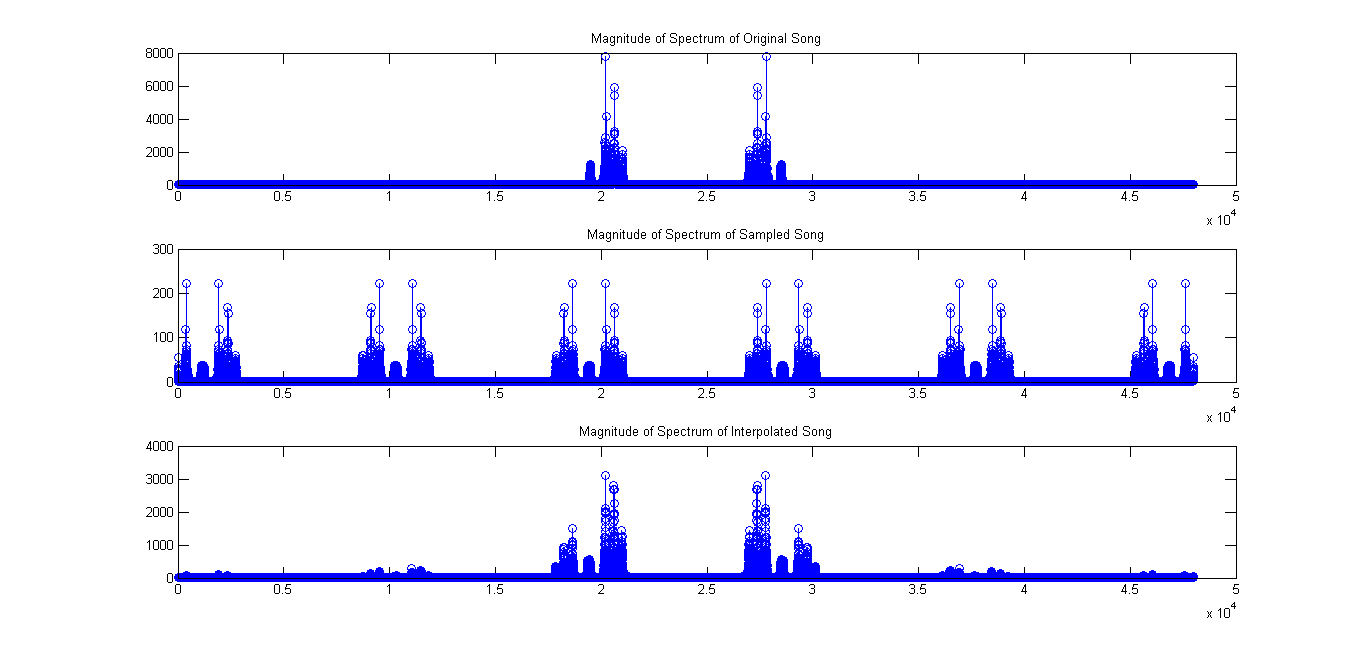
\includegraphics[width = 0.9\textwidth]{p1_n35.png} 

The impulse response for linear interpolation is a triangle of height 1 and width of $2 m + 1$, where $m$ is the interpolation factor. %insert picture here?

As we have seen before in discussion, the triangle function is the convolution of two identical rectangles, and via the convolution theorem, the spectrum of $h[n]$ is a squared sinc.

In interpolation, $Y_s[k]$ is multiplied by $H[k]$ to give us $Y_i[k]$. You can see that the central replica has been distorted by the bell shape of the central sinc lobe. The other replicas are not eliminated as we desire with an ideal low pass filter- they remain nonzero in the side lobes of the squared sinc. 
 
\item [(d)] Now change $N$ to 75 and rerun \texttt{freqMary.m}. What has changed?

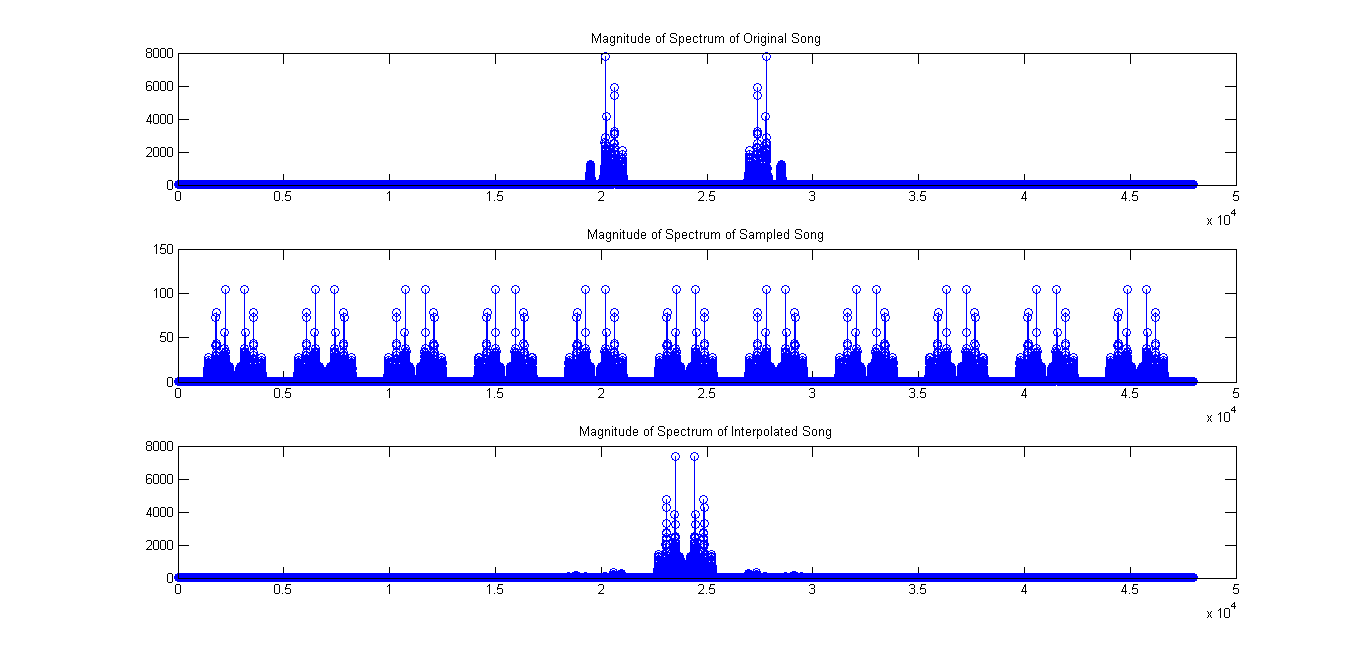
\includegraphics[width = 0.9\textwidth]{p1_n75.png} 

We see significant aliasing of the spectrum. Some of the high frequencies of the shifted replicas are now overlapping with the central replica near the lower frequencies. In fact, the linear interpolation keeps the aliased frequencies, while reducing the energy of the central replica. This can be heard as high notes becoming lower in pitch.

\item [(e)] Submit print outs of plots for both $N=35$ and $N=75$. Also submit your code.

\end{description}






\vspace{5mm}
\item Textbook 8.21 % same number in 3rd edition

\textbf{Solution.} We know from \#7 of Table 8.1 that the multiplication of these two DFS representations, $\widetilde{X}_1[k] \widetilde{X}_2[k]$, is equivalent to performing periodic convolution in the time domain: $$\widetilde{y}_1[n] = \sum_{m=0}^{N-1} \widetilde{x}_1[m] \widetilde{x}_2[n-m]\;.$$ Since one period of $\widetilde{x}_2[n]$ has a delta at $n=2$, we can see that the output will be a shifted version of one period of $\widetilde{x}_1[n]$; we could also perform periodic convolution. Both will result in $\widetilde{y}_1[n]$ as shown in the figure.

  \begin{figure}[htb]
 \centering
 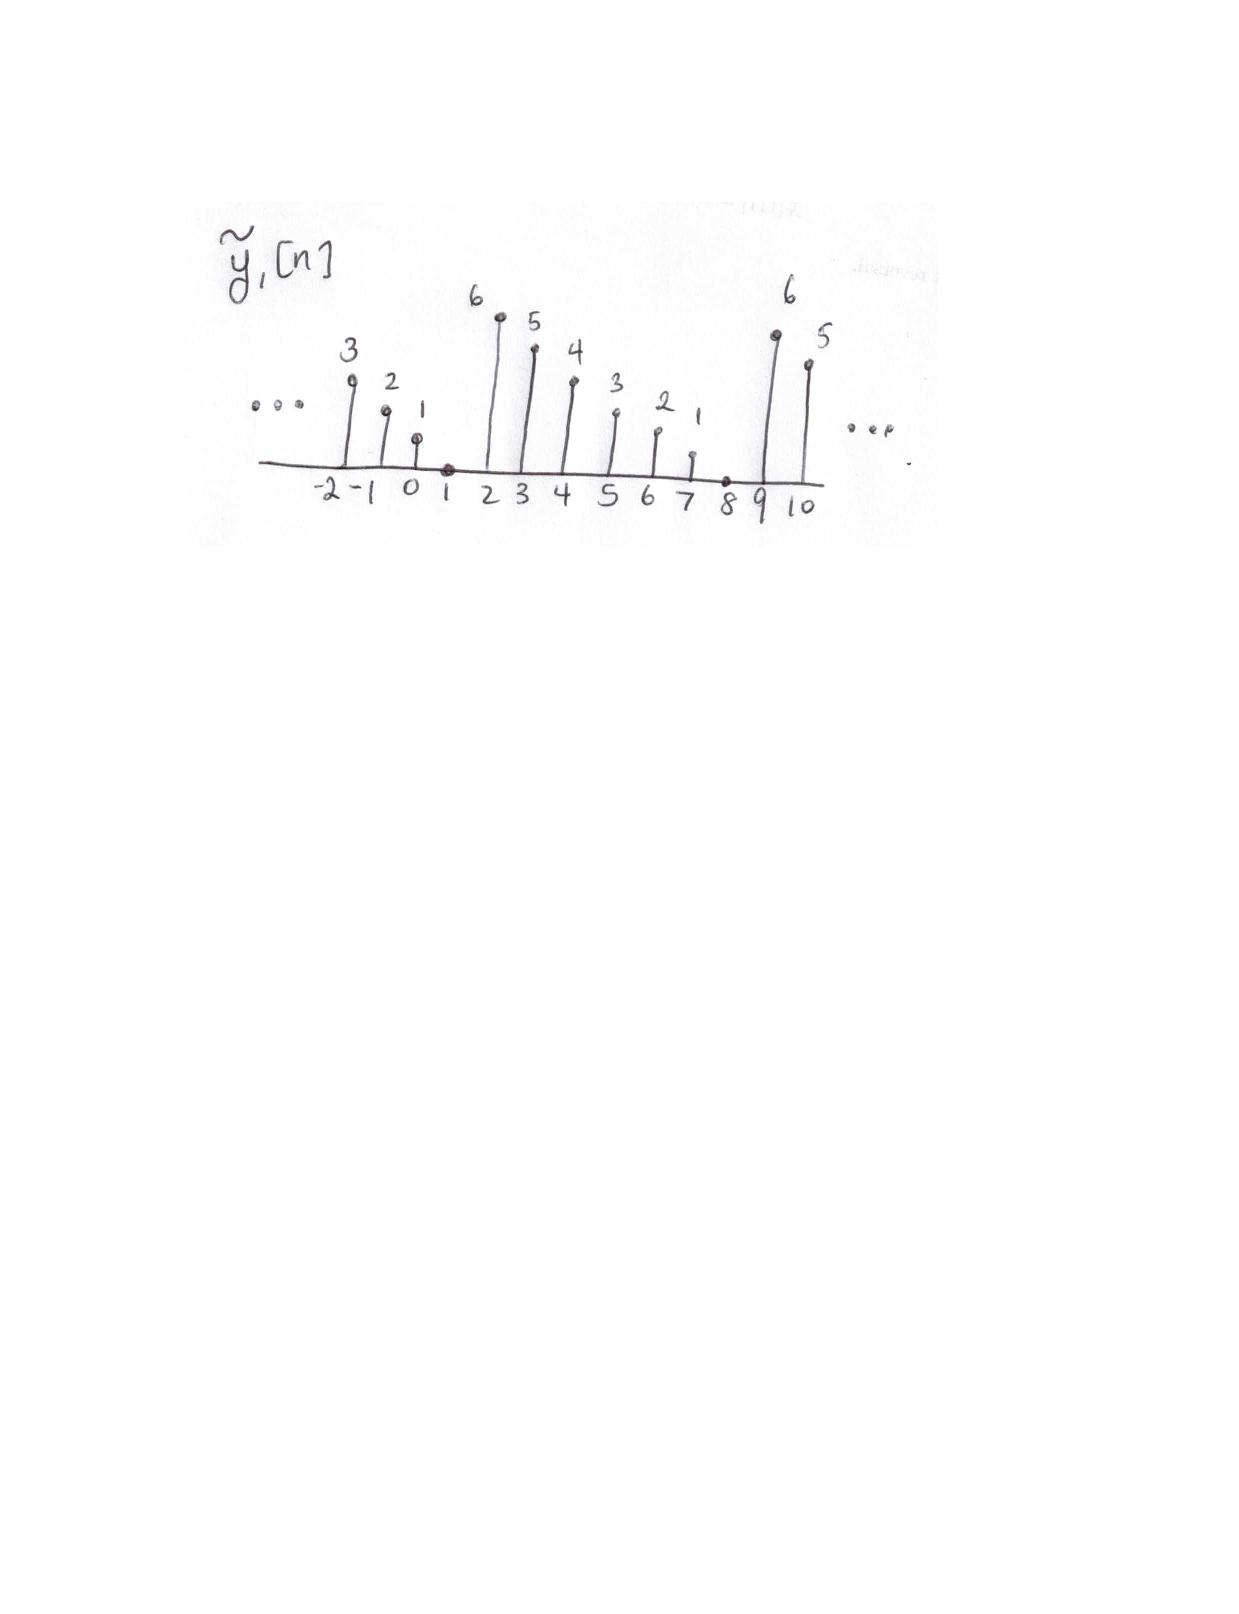
\includegraphics[width=0.5\textwidth]{821periodicconv}
 \end{figure}
 
 We could also compute it by doing multiplication in the frequency domain and converting back to the time domain as follows. $$\widetilde{X}_1[k] = \sum_{n=0}^6 \widetilde{x}_1[n] W_7^{kn} = 6 + 5W_7^k + 4W_7^{2k} + 3 W_7^{3k} + 2W_7^{4k} + W_7^{5k}\;.$$
 
 $$\widetilde{X}_2[k] = \sum_{n=0}^6 \widetilde{x}_2[n] W_7^{kn} = W_7^{2k}\;.$$
 
 $$\widetilde{Y}_1[k] = \widetilde{X}_1[k] \widetilde{X}_2[k] = 6W_7^{2k} + 5W_7^{3k}+4W_7^{4k}+3W_7^{5k}+2W_7^{6k} + W_7^{7k}\;.$$ By our known DFS pairs, we can interpret this for $n=0, \dots, 6$ as $$\widetilde{y}_1[n] = 6\delta[n-2]+5\delta[n-3] + 4\delta[n-4] + 3\delta[n-5] + 2\delta[n] + \delta[n-1]\;;$$ that is, this is one period of $\widetilde{y}_1[n]$, which also matches the figure.
 

\vspace{5mm}
\item Textbook 8.30 %not in 3rd edition

\textbf{Solution Part (a).} We have a delta shifted to 32 in the frequency domain, so we get $$x[n]=\frac{1}{64} e^{-j\frac{2\pi}{64} 32 n} = \frac{1}{64}(-1)^n\;.$$ This is unique because all the values of $\widetilde{X}[k]$ are given.

\textbf{Solution Part (b).} There are two ways to solve this problem. One interprets the given $\widetilde{X}[k]$ as independent of part (a) or the wording at the beginning of the problem, and that we only are given its values on the set $0\leq k \leq 63$. In that case, $$x[n]=\frac{1}{192} e^{-j\frac{2\pi}{192} 32 n} $$ is one possible $x[n]$. Since we don't know what the values of $\widetilde{X}[k]$ are off the set $0\leq k \leq 63$, their values could be consistent with a different $x[n]$, for example the same $x[n]$ as part (a); then we would also have $\widetilde{X}[96]=1$ and $\widetilde{X}[160]=1$. 

\vspace{4mm} The second interpretation has similar results. Here we interpret the wording ``consistent with the constraint'' as to refer to the samples of the DTFT given above part (a). Since the $x[n]$ of part (b) will have 3 times as many samples, we assume to be ``consistent'' with part (a) means to match on every third sample. That means that this new frequency domain sequence, call it $
\widetilde{X}_b[n]$, has $\widetilde{X}_b[3k] = \widetilde{X}[k]$ from the earlier definition of $\widetilde{X}[k]$, and therefore $\widetilde{X}_b[96]=1$ and $\widetilde{X}_b[3k]=0$ for other $k = 0, \dots, 63$. In that case, an $x[n]$ that would work would be $$x[n] = \frac{1}{192} e^{-j\frac{2\pi}{192} 96 n} = \frac{1}{192}(-1)^n\;.$$ However, as in the above interpretation, the rest of the values $\widetilde{X}_b[m], m \neq 3k$ could be anything, and so there are many other $x[n]$ that could work.

\vspace{5mm} 
\item Textbook 8.67 % 8.70 in 3rd edition

\begin{description}
\item[(a) extra-credit] Since $V(e^{j\omega}) = X(e^{j 4 \omega})$, we desire to have a low pass filter that has the following magnitude:

\[ |H(e^{j\omega}| = \begin{cases}1, &|\omega| \leq \frac{\pi}{4} \\ 0, & \text{otherwise} \end{cases} \]

Since $h[n]$ is FIR, we assume it is non-zero over $0 \leq k \leq N$. The phase of $H(e^{j \omega)}$ should be set such that $h[n]$ is symmetric about the center of its range, i.e. $\frac{N}{2}$. Therefore, the phase of $H(e^{j\omega})$ should be $e^{j \omega \frac{N}{2}})$. Then the $4N$-point DFT of $h[n]$ is:

\[ H[k] = H(e^{j \omega})\big|_{\omega = \frac{2 \pi k}{4N}} = \begin{cases} e^{j \frac{\pi}{4}k}, & 0 \leq k \leq \frac{N}{2} \\ 0, & \frac{N}{2} \leq k \leq 4N-\frac{N}{2} - 1 \\ e^{j \frac{\pi}{4}} k, & 4N -\frac{N}{2} \leq k \leq 4N \end{cases}\]

Note to graders: Since we did not talk specifically in class about whether the convention is to place the extra odd sample on the left or the right of zero, we will also accept $0\leq k \leq \frac{N}{2}+1$ as the range for the first segment if $4N-\frac{N}{2}+1 \leq k \leq 4N$ is the range for the third segment.

\item[(b)] This part asks to design System $A$.

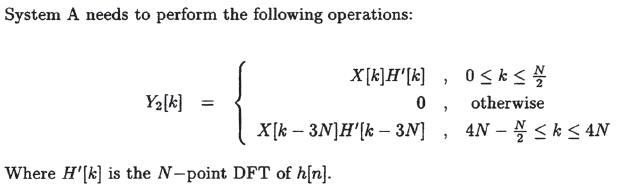
\includegraphics[width = 0.9\textwidth]{8_70b_soln.png} 

Note to graders: Since we did not talk specifically in class about whether the convention is to place the extra odd sample on the left or the right of zero, we will also accept $0\leq k \leq \frac{N}{2}+1$ as the range for the first segment if $4N-\frac{N}{2}+1 \leq k \leq 4N$ is the range for the third segment.

\item[(c)] It is cheaper to implement $N$-point DFTs than $4N$-point DFTs, therefore the implementation for part a is preferable to that in part b. We can replace a $4N$-point DFT of $v[n]$ with an $N$-point DFT of $x[n]$. (Additionally, we can replace $4N$-point DFT $H[k]$ with $N$-point DFT $H'[k]$. However, the savings from that switch are less dramatic, as the filter is often applied to multiple signals and so we precompute its DFT.)
\end{description}

\vspace{5mm} 
\item The deterministic crosscorrelation function between two real sequences is defined as
% 8.49 in 3rd edition

\[
c_{xy}[n]=\sum_{m=-\infty}^\infty y[m]x[n+m] = \sum_{m=-\infty}^\infty y[-m]x[n-m]=y[-n]*x[n]\quad -\infty < n < \infty
\]

\begin{description}
\item[\textbf{(a)}] Show that the DTFT of $c_{xy}[n]$ is $C_{xy}(e^{j\omega}) = X(e^{j\omega})Y^*(e^{j\omega})$.

\textbf{Solution.} We know that the DFTF of a convolution is the product of the DTFTs; i.e. if $y[-n] = \widetilde{y}[n]$ we have $$C_{xy}(\omega) = X(\omega) \widetilde{Y}(\omega)\;.$$ To finish this off, we note that since $y[n]$ is real, the DTFT of $y[-n]$ is $Y^*(\omega)$. 

\item[\textbf{(b)}] Suppose that $x[n] = 0$ for $n < 0$ and $n > 99$ and $y[n]=0$ for $n < 0$ and $n > 49$. The corresponding crosscorrelation function $c_{xy}[n]$ will be nonzero only in a finite-length interval $N_1 \leq n \leq N_2$. What are $N_1$ and $N_2$?

\textbf{Solution.} From what we know about convolution, we know that $c_{xy}[n]$ will have length of $50+100-1 = 149$ samples. Considering flip and shift, we can see that $N_1 = -49$ and $N_2=99$. 

\item[\textbf{(c)}] Suppose that we wish to compute values of $c_{xy}[n]$ in the interval $0 \leq n \leq 20$ using the following procedure:
\begin{description}
\item[\textbf{(i)}] Compute $X[k]$, the $N$-point DFT of $x[n]$
\item[\textbf{(ii)}] Compute $Y[k]$, the $N$-point DFT of $y[n]$
\item[\textbf{(iii)}] Compute $C[k]=X[k]Y^*[k]$ for $0 \leq k \leq N - 1$
\item[\textbf{(iv)}] Compute $c[n]$, the inverse DFT of $C[k]$
\end{description}
What is the \textit{minimum} value of $N$ such that $c[n] = c_{xy}[n]$, \\$0 \leq n \leq 20$? Explain your reasoning.


\textbf{Solution.} Since we want $c[n]$ to equal $c_{xy}[n]$ for $0\leq n \leq 20$, we need to make sure that the convolution has no aliasing in that range. Therefore we must choose $N\geq100$. See Figure~\ref{fig:crosscor} for an illustration.  Note that this actually gets $c[n] = c_{xy}[n]$ for $0\leq n \leq 49$.

\begin{figure}[htb]
 \centering
 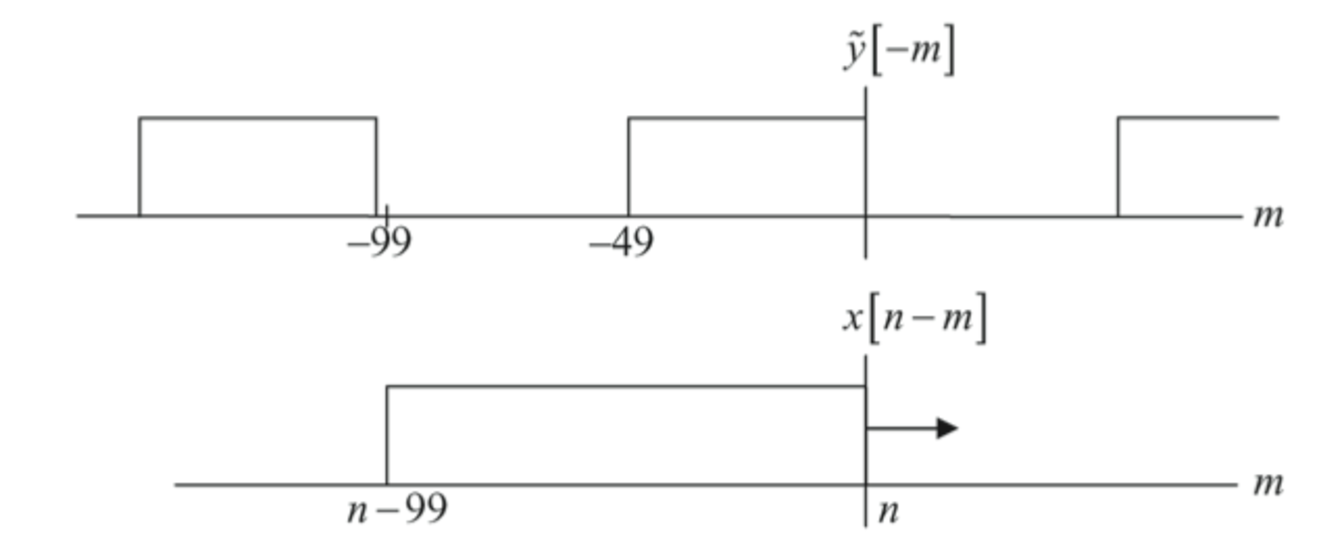
\includegraphics[width=1\textwidth]{crosscorrDFTconv}
 \caption{Picture for \#5 Part (c).}
 \label{fig:crosscor}
 \end{figure}

\end{description}


\end{enumerate}


\end{document}